% Created 2022-12-27 Ter 23:00
% Intended LaTeX compiler: pdflatex
\documentclass[a4paper]{article}
\usepackage[utf8]{inputenc}
\usepackage[T1]{fontenc}
\usepackage{graphicx}
\usepackage{longtable}
\usepackage{wrapfig}
\usepackage{rotating}
\usepackage[normalem]{ulem}
\usepackage{amsmath}
\usepackage{amssymb}
\usepackage{capt-of}
\usepackage{hyperref}
\usepackage[margin=0.8in]{geometry}
\author{Davi Raubach Tuchtenhagen}
\date{\today}
\title{Pré-composição\\\medskip
\large Oficina de Música de Curitiba 2023}
\hypersetup{
 pdfauthor={Davi Raubach Tuchtenhagen},
 pdftitle={Pré-composição},
 pdfkeywords={},
 pdfsubject={},
 pdfcreator={Emacs 29.0.50 (Org mode 9.5.4)}, 
 pdflang={English}}
\begin{document}

\maketitle

\section*{Pré-composição}
\label{sec:org98ea351}
\subsection*{Intro}
\label{sec:org950ad23}
Entendo a pré-composição como um momento de trabalho imaginativo que se direciona para vários âmbitos. Esta imaginação, enquanto capacidade de gerar "imagens" que ultrapassam a realidade, toma a instrumentação, a notação, a performance, as estruturas (alturas, ritmos, texturas, etc.) como material. O poeta Manuel de Barros escreveu que "o olho vê, a memória revê e a imaginação transvê". Neste momento, mudo e mudo novamente a direção de meu olhar no objetivo de transver estes elementos para uma futura implementação na composição. Minha transvisão da performance/notação já foi apresentada na submissão da proposta. Me refiro à utilização da leitura de um texto verbal associada à leitura musical. Esta proposta se desdobra, agora, na ideia de definir diferentes estilos de leitura. Por exemplo, ao escrever um ritornelo de um material sobre um texto, indicar diferentes estilos de leitura para um mesmo texto. Os tipos que me ocorreram foram: protesto, poético, sabedoria.

Exemplos:
\begin{itemize}
\item Protesto: leitura intensa (mais rápido e com rompantes): \url{https://youtu.be/6\_uYWDyYNUg?t=57}
\item Poético / Neruda (lento e ritmado): \url{https://youtu.be/6KclpaxCYUw}
\item Sabedoria (lento e com pausas): \url{https://youtu.be/fZXhPmHPoNo?t=98}
\end{itemize}

Uma transcrição em notação tradicional rítmica deve ser feita de uma frase para cada estilo para exemplificar o tipo de leitura a ser feito. Esboço abaixo:

\begin{center}
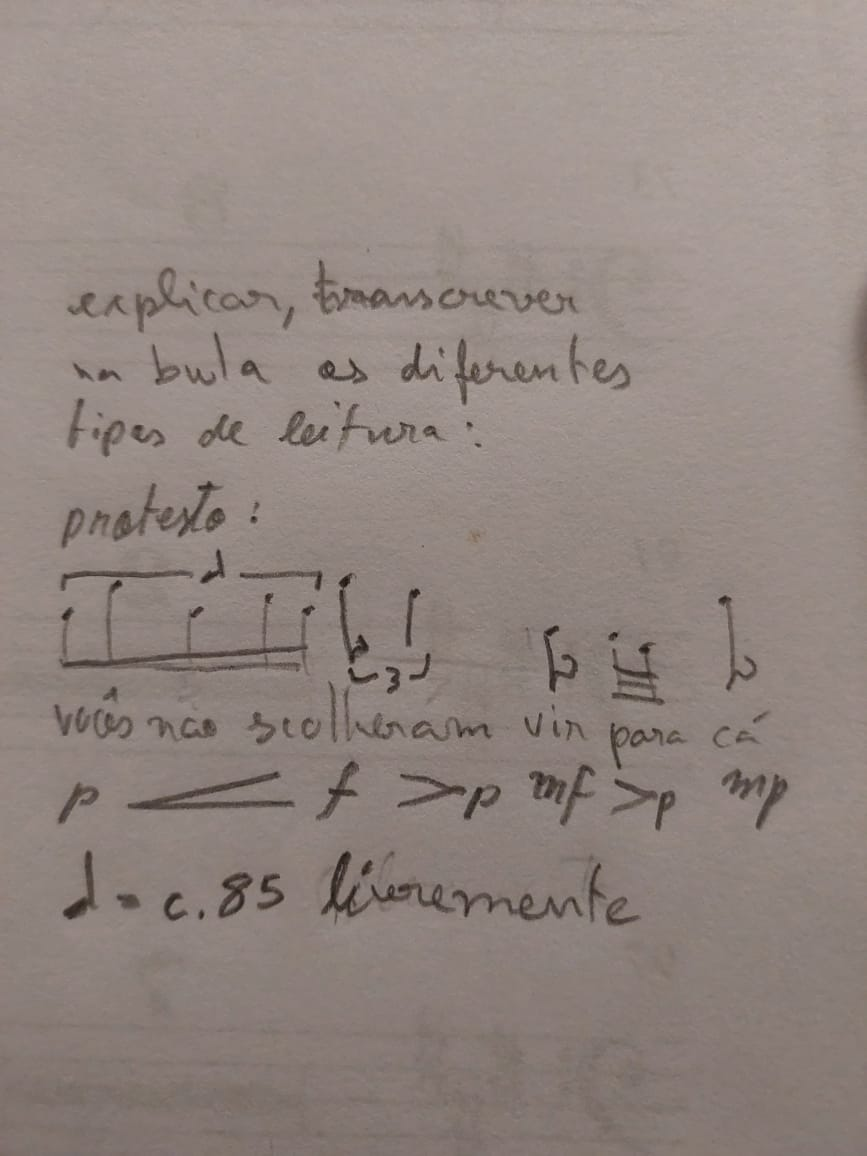
\includegraphics[width=5cm]{exemploprotesto.jpeg}
\end{center}

Os estilos distintos podem ajudar os intérpretes a se engajar mais na busca de um resultado interessante.

Outra ideia é utilizar réguas temporais diferentes para os instrumentos. Por exemplo: Violão toca material musical associado à leitura de um texto e os demais tocam materiais musicais associados aos materiais do violão. Seria preciso pensar com certo delay as partes relativas para que haja tempo para perceber o que o colega está tocando e então tocar a sua parte. Estimula a escuta no grupo.

\subsection*{Multifônicos / alturas}
\label{sec:orgae2937a}
A ideia dos multifônicos como elemento para derivar alturas estava presente na minha última peça e também é um contágio da proposta do Charles Neimog. Escolhi os seguintes, mas preciso conferir com o Sérgio.

\subsubsection*{Sax soprano}
\label{sec:org7b67ee9}
Multi1:
\begin{center}
\includegraphics[width=5cm]{images/Captura de Tela 2022-12-27 às 16.45.54.png}
\end{center}

Multi2:
\begin{center}
\includegraphics[width=5cm]{images/Captura de Tela 2022-12-27 às 16.44.20.png}
\end{center}

Retirados de WEISS, Marcus; NETTI, Giorgio. The techniques of saxophone playing. Bärenreiter, 2010.

\begin{itemize}
\item Modulação
\label{sec:org2738d7c}
Modulação para geração de alturas derivadas do multifônico. Para cada duas frequências (A e B) do multifônico, as seguintes são geradas:

\begin{itemize}
\item FreqB - FreqA
\item FreqB + FreqA
\item 2x FreqB + FreqA
\item 2x FreqB - FreqA
\item 2x FreqA + FreqB
\item 2x FreqA - FreqB
\end{itemize}

Código Python:
\begin{verbatim}
import muda
multi_1 = [6.75, 8, 20, 27, 29, 31] # notas originais
multi_1_mod = muda.ring_modulation(multi_1) # modulação
multi_1_mod.sort() # organiza do grave para o agudo
multi_1_mod = list(dict.fromkeys(multi_1_mod)) # remove repetidas
# muda.see_pitches(multi_1_mod) # gera ilustração

multi_2 = [11, 12, 23, 30.5]
multi_2_mod = muda.ring_modulation(multi_2)
multi_2_mod.sort()
multi_2_mod = list(dict.fromkeys(multi_2_mod)) 
# muda.see_pitches(multi_2_mod)

\end{verbatim}

Multi1 modulado:
\begin{center}
\includegraphics[width=.9\linewidth]{images/Captura de Tela 2022-12-27 às 17.21.23.png}
\end{center}


Multi2 modulado:
\begin{center}
\includegraphics[width=.9\linewidth]{images/Captura de Tela 2022-12-27 às 17.31.00.png}
\end{center}
\end{itemize}


\subsection*{Forma}
\label{sec:org6da7b34}
Além da duração (entre 3 e 4 min), não pude conceber, de maneira geral, como será a forma da peça. E, na verdade, não gostaria de fazer isso. Desta vez, assim como foi com "Atrás do vento" (\url{https://www.youtube.com/watch?v=qvdGW\_YyjpM}), vou trabalhar um pouco mais "de ouvido", consultando a música antes de prosseguir.

É certo dizer que buscarei um decorrer semelhante a outras peças recentes em que quase tudo é gradação. Processos de alternâncias de materiais fazem a peça ir de um ponto a outro aos poucos. É um rio.

Alternância de materiais \emph{a}, \emph{b,} e \emph{r:}
\begin{center}
\includegraphics[width=.9\linewidth]{/Users/davi/Composição/2022/Plurisons/timespans.png}
\end{center}


\subsection*{Começo}
\label{sec:orgd8829f3}
c. 1:30

Agudíssimo. Piccolo + Violão. Violão com slide em região super aguda em contraponto rítmico com piccolo. Forte. Cello em paralelo toca ressonância destas notas com variação sul pont. sul tasto. Sax soprano toca multifônicos filtrados, buscando as notas agudas (usar as mesmas para piccolo, violão e cello).

Abaixo, a partitura (ainda errada) do início deste trecho. Aqui utilizei o segundo multifônico. A ideia é trabalhar com transição de um espectro de alturas para outro ao mesmo tempo em que há preenchimento gradual da região grave.

Decidi apresentar a partitura com notação rítmica tradicional para demonstrar que estou tentando "espacializar" a escrita. Isto é, não deixar somente a cargo da leitura, mas também apresentar o texto de maneira espaçada para sugerir leituras diferentes.

Posteriormente, os "engravers" são removidos (beams, dots, barlines, etc.) se assemelhando mais a pauta do piccolo.

Tarefas:
\begin{itemize}
\item Melhorar a notação do multifônico
\item Melhorar relação texto-música
\item Indicar estilo de leitura
\end{itemize}

\begin{center}
\includegraphics[width=.9\linewidth]{images/Captura de Tela 2022-12-27 às 22.38.20.png}
\end{center}
\end{document}